\section{Kos}\label{kos}

Tags: Città, Sede Gilda Creatore: Lorenzo Ispirazione: Cosenza

\section{Kos}\label{kos-1}

\begin{center}\rule{0.5\linewidth}{0.5pt}\end{center}

\begin{figure}
\centering
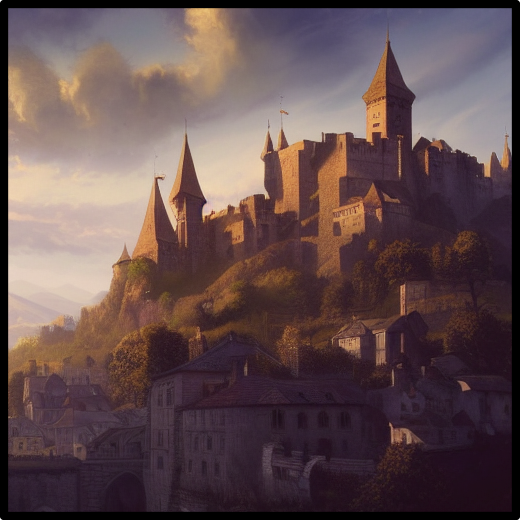
\includegraphics{Untitled.png}
\caption{Untitled}
\end{figure}

Informazioni Generali

Tipo di luogo: Città-Stato

Dimensioni: 48,71 km²

Altitudine: 238 m s.l.m.

Popolazione: 100.000

Paese: Valtara

Alleata con:

Attività:

\begin{center}\rule{0.5\linewidth}{0.5pt}\end{center}

\subsection{1. Descrizione Generale}\label{descrizione-generale}

\begin{center}\rule{0.5\linewidth}{0.5pt}\end{center}

\begin{figure}
\centering
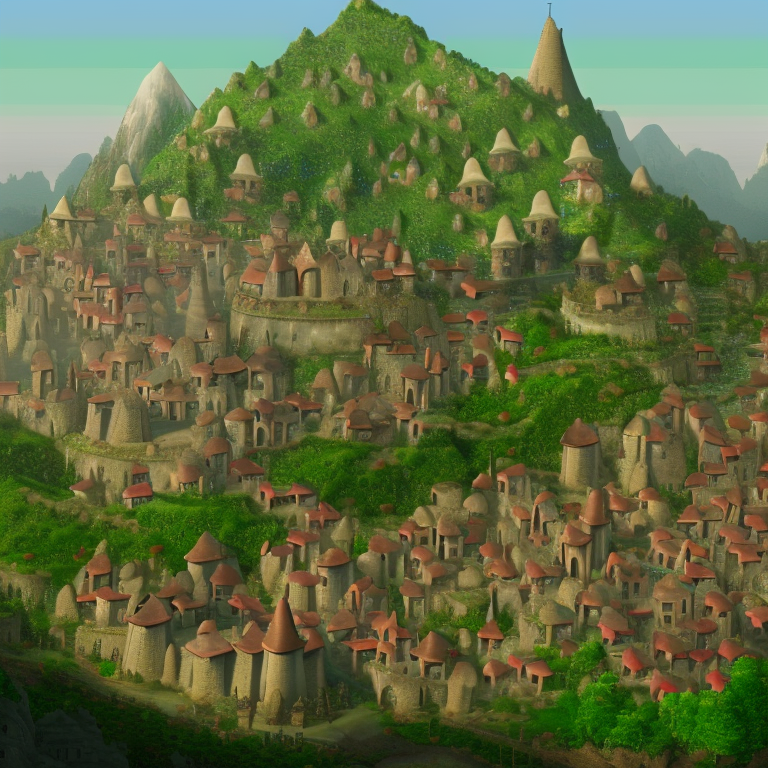
\includegraphics{a-large-medieval-city-in-a-mountain-area--.png}
\caption{Dipinto di Kos risalente a circa 500 anni fa}
\end{figure}

Dipinto di Kos risalente a circa 500 anni fa

Kos è una città stato indipendente situata su una collina non molto
distante dalle montagne, circondata dal fiume Kratos. Il paesaggio è
caratterizzato da boschi e prati, che si estendono fino alle montagne e
in tutta la zona circostante. La città è costruita principalmente in
pietra. Le case sono generalmente a due o tre piani, con pareti spesse e
finestre a croce. Molte case hanno anche un cortile interno con un pozzo
centrale, dove le famiglie possono raccogliere acqua per il loro uso
quotidiano. Le case più antiche e le case signorili della città sono
dotate di dettagli architettonici più elaborati, come archi, cornici
scolpite e finestre a bifora. Inoltre, molte case hanno anche piccole
torri o campanili che conferiscono loro un aspetto maestoso.

\begin{quote}
\textbf{``Va coglia riganu ara scisa i Paö L'And'' - detto popolare nel
dialetto di Kos}
\end{quote}

\subsection{2. Storia}\label{storia}

\begin{center}\rule{0.5\linewidth}{0.5pt}\end{center}

La città nasce tra (?), dall'aggregazione delle popolazioni dei piccoli
villaggi tra le montagne e il Kratos, che videro nella collina di Kos il
luogo ideale dove stabilirsi. Nel corso dei secoli successivi, Kos
divenne un punto di riferimento commerciale per tutta la regione della
Foresta dei Giganti, che divenne una delle zone più floride dell'intera
Valtara.

Durante i decenni ricordati ancora oggi dagli abitanti come il periodo
delle ``\emph{Pezze aru culu}'', un tiranno conosciuto come Zorvan il
Terribile soggiogò la città e i suoi abitanti. Il tiranno poteva contare
su un fidato esercito di suoi seguaci, a cui permetteva di prendere ciò
che desideravano dalla popolazione, senza alcun pietà o compassione. La
città fu sottoposta a una pesante tassazione, le strade furono rese
insicure e il commercio quasi si arrestò.

Nonostante ciò, alcuni coraggiosi abitanti di Kos, guidati da un ordine
di paladini nato con l'obiettivo di far cadere il governo del tiranno,
si organizzarono in segreto per resistere alla dominazione di Zorvan e
dei suoi sgherri. Cominciarono a pianificare azioni di guerriglia e a
sabotare i rifornimenti del tiranno. Questa resistenza segreta riuscì a
sopravvivere anche quando sembrava che tutto fosse perduto, e iniziò a
ottenere il supporto di sempre più persone che si ribellavano contro le
ingiustizie. Dopo anni di resistenza, i paladini entrarono in città con
un esercito di cittadini valorosi, e insieme sconfissero il terribile
dittatore.

{[}500 anni prima gli eventi delle nostre avventure{]}

Da allora, la città di Kos si è sempre impegnata nel difendere la sua
libertà e la sua indipendenza.

Nel periodo successivo alla guerra, Kos conobbe un periodo di
rinnovamento e sviluppo. Furono costruiti nuovi edifici pubblici, strade
più larghe e moderne, e la città divenne un importante centro culturale
grazie alla presenza di scuole, biblioteche e musei.

Oggi, Kos è una città fiorente e prospera, con una forte economia basata
sul commercio e sull'artigianato.

\subsection{3. Geografia}\label{geografia}

\begin{center}\rule{0.5\linewidth}{0.5pt}\end{center}

\subsubsection{3.1 Distretti}\label{distretti}

\begin{center}\rule{0.5\linewidth}{0.5pt}\end{center}

\begin{figure}
\centering
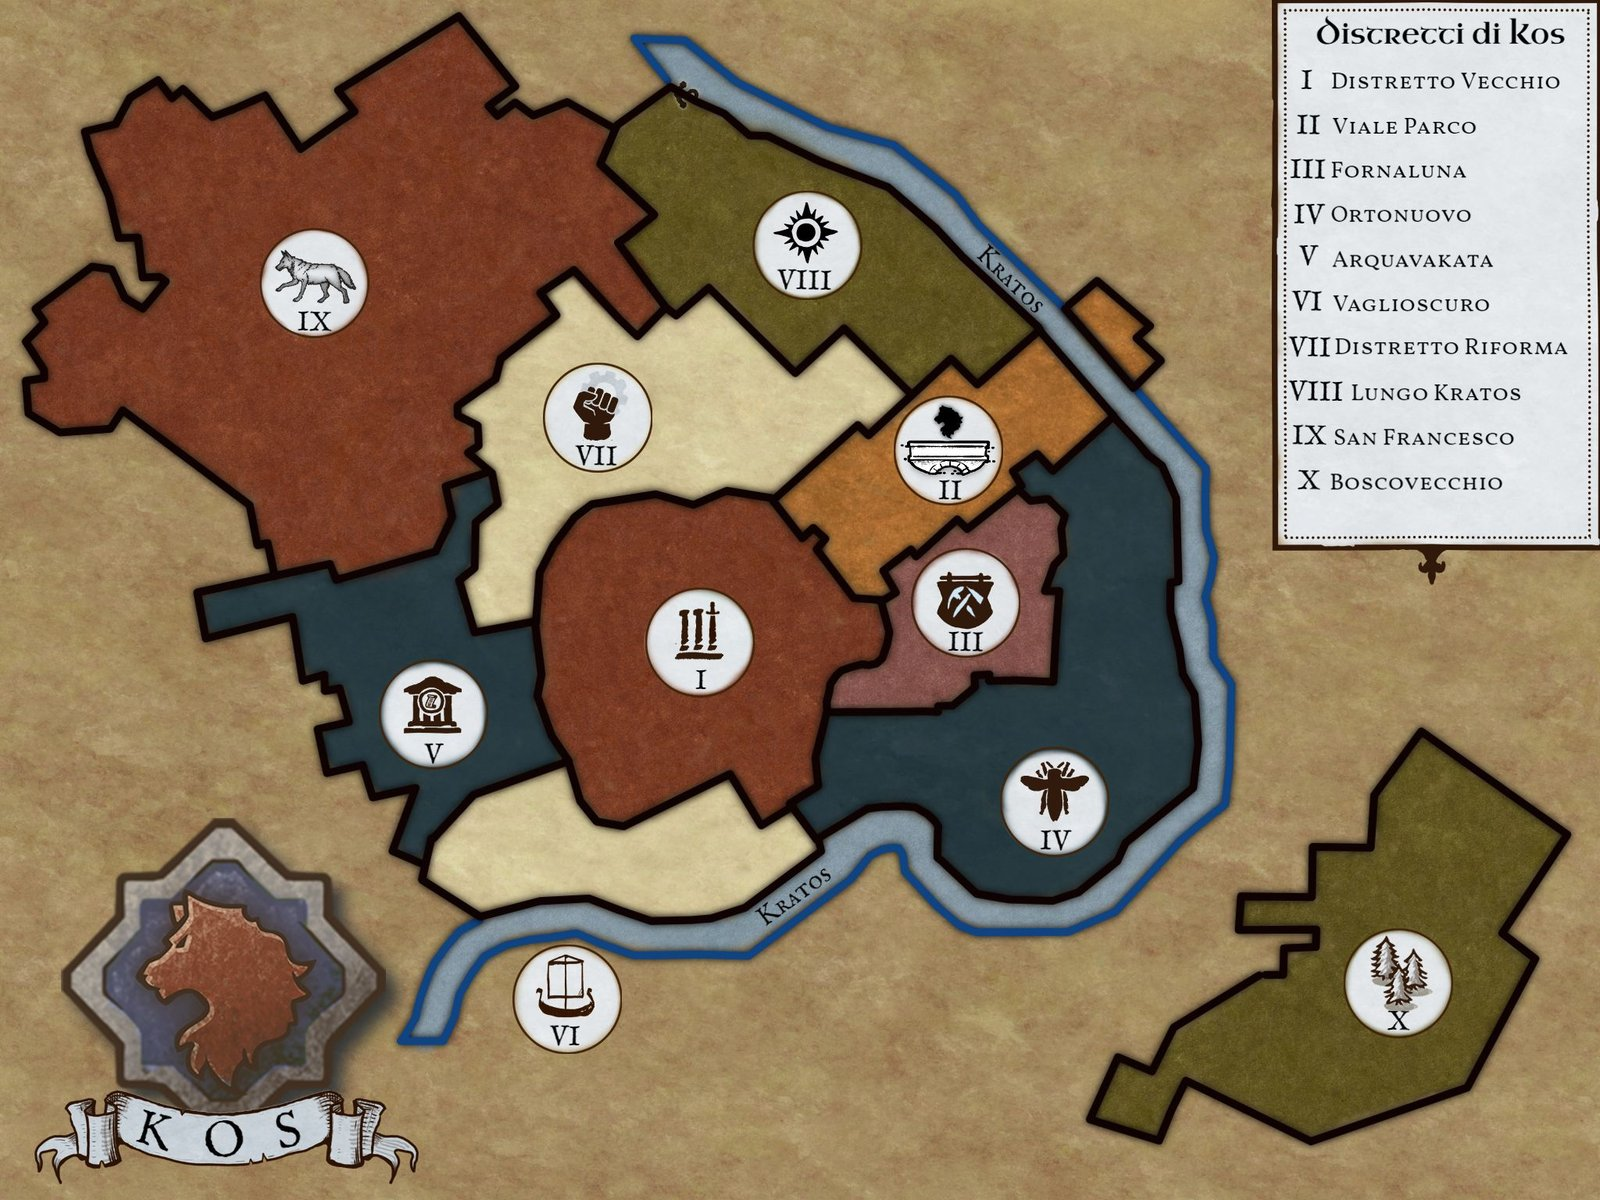
\includegraphics{distretti_kos.jpg}
\caption{distretti kos.jpg}
\end{figure}

La città di Kos è divisa in 10 distretti:

\begin{enumerate}
\def\labelenumi{\arabic{enumi}.}
\tightlist
\item
  \textbf{Distretto Vecchio}: abitato principalmente da famiglie di
  origini aristocratiche, i cui membri gestiscono attività commerciali e
  artigianali di prestigio nella città. La popolazione del Centro
  Storico è molto variegata, composta da mercanti, artisti, politici e
  intellettuali.
\item
  \textbf{Viale Parco}: distretto che si estende dal centro città fino a
  valle, superando il fiume Kratos. Questo distretto è noto per il lungo
  viale alberato che collega le porte della città al suo centro storico.
  Il distretto è abitato principalmente da famiglie di commercianti
  molto impegnate per garantire la prosperità della città. Il viale
  alberato del distretto viene chiuso annualmente per ospitare la grande
  fiera di San Josephus.
\item
  \textbf{Fornaluna}: distretto dell'artigianato. Famoso per le numerose
  botteghe del legno che espongono le loro opere lungo le strette vie
  del quartiere.
\item
  \textbf{Ortonuovo}: questo distretto abitato da famiglie della classe
  media e lavoratori dipendenti. Qui le case sono più modeste, ma la
  vita è tranquilla e le strade sono molto pulite. La popolazione è
  molto varia.
\item
  \textbf{Arquavakata}: centro della magia e della conoscenza, noto
  principalmente per la presenza dell'università. Abitato da studiosi di
  ogni sorta, ricercatori e intellettuali. La popolazione qui è molto
  attenta alla cultura e alle arti, e partecipa attivamente a eventi
  culturali nella città.6
\item
  \textbf{Vaglio Scuro}: ****distretto importante per la presenza del
  porto, dove attraccano le navi che, navigando sul Kratos, portano
  merci e spezie alla città.
\item
  \textbf{Distretto Riforma}: distretto centrale della città, deve il
  suo nome alla riforma che portò alla creazione del Consiglio
  Cittadino, permettendo al popolo di essere partecipe alle decisioni
  politiche della città.
\item
  \textbf{LungoKratos}: distretto residenziale che si estende lungo la
  sponda del fiume.
\item
  \textbf{Distretto San Francesco}: nonostante il nome, questo è il
  distretto più problematico della città, dove organizzazioni malavitose
  gestiscono la maggior parte delle attività. La popolazione più
  indigente vive qui, e spesso non ha gli strumenti per uscire dal giogo
  della criminalità.
\item
  \textbf{Boscovecchio}: Questo quartiere è abitato principalmente da
  nani e mezzi nani boscaioli noti per la loro abilità nella lavorazione
  del legno. La popolazione è molto legata alla Foresta dei Giganti che
  circonda la città, e la sua cultura è fortemente influenzata dalle
  tradizioni della comunità dei nani boscaioli.
\end{enumerate}

\subsection{4. Demografia}\label{demografia}

\begin{center}\rule{0.5\linewidth}{0.5pt}\end{center}

\begin{figure}
\centering
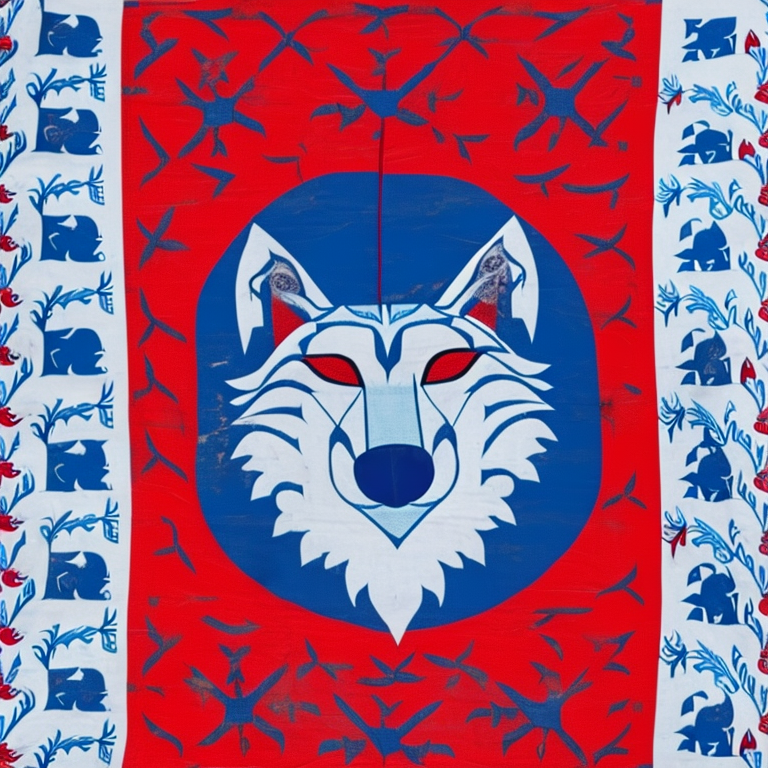
\includegraphics{a-medieval-banner-blue-and-red-colours-depicting-a-wolf-.png}
\caption{Stemma della città di Kos}
\end{figure}

Stemma della città di Kos

La città di Kos ha una popolazione di circa 70.000 abitanti, ed è
composta principalmente da famiglie di commercianti e artigiani. Kos è
stata tradizionalmente un importante centro di commercio e di scambi, e
questa attività ha contribuito alla diversità culturale e razziale della
città. Nonostante la grande diversità, il sentimento di appartenenza è
molto forte e spesso eccessivamente manifestato dai suoi abitanti.

La maggioranza della popolazione è di sangue misto (30\%),
principalmente mezzi nani, dovuto alle migrazioni dei nani boscaioli,
che scesero dalle montagne a valle per la lavorazione del legno.

\begin{quote}
\emph{``La gente di Kos è coraggiosa e leale, pronta a difendere la
propria città e i propri diritti''}
\end{quote}

\subsection{5. Economia}\label{economia}

\begin{center}\rule{0.5\linewidth}{0.5pt}\end{center}

Kos è un centro commerciale vitale nella regione, grazie alla sua
posizione strategica lungo il fiume Kratos una delle rotte commerciali
principali della regione. Questo fa del commercio l'attività chiave
della città: i mercanti viaggiano da e per Kos, portando con sé merci
proveniente da altre città. L'artigianato è un'altra attività economica
importante per la città. I produttori locali creano tessuti, ceramiche e
altri prodotti artigianali che vengono venduti nei negozi della città ed
esportati dei mercanti in tutta la regione. Inoltre, la città ha una
lunga tradizione nella lavorazione del legno. La città si trova nel
cuore della Foresta dei Giganti, area boschiva estesa che ospita alberi
secolari di diverse specie, tra cui querce, castagni e faggi. Grazie
alla qualità del legno proveniente da questa foresta, gli artigiani
locali possono creare mobili, strumenti musicali, oggetti di artigianato
e altri prodotti di legno di alta qualità. La lavorazione del legno è
una tradizione che risale a lungo nella storia di Kos, e ci sono ancora
molti artigiani locali che continuano a praticare questa arte. Inoltre,
la città ha anche una scuola di artigianato del legno che insegna le
tecniche di lavorazione del legno ai giovani e ai turisti interessati.
La lavorazione del legno non è solo un'attività economica importante per
la città, ma anche un'attrazione turistica. Molti visitatori vengono a
Kos per ammirare la bellezza degli oggetti di legno fatti a mano e
acquistarli come souvenir.

\subsection{6. Cultura}\label{cultura}

\begin{center}\rule{0.5\linewidth}{0.5pt}\end{center}

\subsubsection{6.1 Cucina}\label{cucina}

La città di Kos è famosa in tutta la regione per le sue prelibatezze,
fra le quali si annoverano le patate appiccicose di Totonno Uskualu, la
frittata senza uova di Riviero il Freddo e le polezze di San Josephus.

\subsubsection{6.2 Ricorrenze}\label{ricorrenze}

Ogni anno, la città ospita la Fiera di San Josephus, l'evento più atteso
dell'anno, in cui i mercanti di tutta la regione accorrono in città per
vendere le loro merci e fare affari. La fiera trasforma Kos in un luogo
di festa e di fermento, con le sue strade affollate di persone
provenienti da ogni angolo di Valtara. Gli artigiani locali espongono le
loro opere in bancarelle colorate, mentre i mercanti viaggiano da
lontano per vendere spezie, tessuti e oggetti rari provenienti da terre
lontane.

\begin{center}\rule{0.5\linewidth}{0.5pt}\end{center}

\subsection{7. Governo}\label{governo}

\begin{center}\rule{0.5\linewidth}{0.5pt}\end{center}

Kos viene governata dal Consiglio cittadino, i cui membri sono:

\begin{itemize}
\tightlist
\item
  2 rappresentanti per ogni distretto, detti Rappresentanti Distrettuali
  ed eletti dal popolo;
\item
  7 esponenti delle famiglie commerciali più importanti, detti
  Consiglieri, scelti arbitrariamente dal Moderatore in base alla loro
  influenza economica, la loro reputazione e le opere compiute per la
  comunità;
\item
  1 Moderatore, eletto ogni 5 anni dai Rappresentanti distrettuali.
\end{itemize}

Il ruolo dei Consiglieri è quello di formulare le politiche che
riguardano ogni aspetto della città. Il ruolo dei Rappresentanti
Distrettuali è quello di votare le proposte dei Consiglieri. Se le
proposte ottengono la loro approvazione, diventano leggi. Il Moderatore,
oltre a scegliere i Consiglieri, ha il compito di regolare gli incontri
del Consiglio. Inoltre ha l'ultima parola in caso di stallo nelle fase
di approvazione delle leggi.

\subsection{8. Organizzazioni}\label{organizzazioni}

\begin{center}\rule{0.5\linewidth}{0.5pt}\end{center}

\begin{itemize}
\tightlist
\item
  \textbf{Gilda dei Mercanti}: si occupa principalmente della
  regolamentazione e del controllo del commercio all'interno della
  città, oltre a gestire le relazioni commerciali con altre città e
  paesi. I suoi membri sono principalmente commercianti, mercanti e
  banchieri, e la gilda ha un ruolo importante nell'economia della
  città, poiché promuove l'attività commerciale e garantisce la corretta
  applicazione delle leggi commerciali e fiscali. Il capo della gilda è
  di diritto uno dei Consiglieri del Consiglio Cittadino.
\item
  \textbf{Gilda dei Giganti}: nonostante il nome, la Gilda dei Giganti è
  stata fondata dai nani boscaioli per normare ogni passaggio della
  lavorazione del legno, dall'abbattimento dell'albero, alla vendita dei
  prodotti di artigianato. La gilda include falegnami, intagliatori,
  ebanisti e altri artigiani specializzati nella lavorazione del legno.
  La gilda è responsabile di garantire la qualità del legno e dei
  prodotti finiti e di promuovere la conoscenza e le tecniche di
  lavorazione del legno.~ Inoltre, la Gilda dei Giganti a Kos è spesso
  coinvolta nella gestione della foresta dei giganti, assicurando la
  sostenibilità delle risorse e proteggendo l'ambiente.
\item
  \textbf{Gilda dei Protettori della Sila Devoti a San Francesco e ai
  Lupi}: Kos è la città natale di questa rinomata Gilda di avventurieri.
\item
  \textbf{Nera Gandatha}: è una gilda criminale strutturata e ben
  amalgamata alla città. Oltre alle attività criminali più classiche,
  come estorsioni, l'usura o il commercio di beni illegali (attività che
  conduce solo nei quartieri più periferici della città, lontani dagli
  occhi della Kos ben pensante), la gilda cerca di infiltrarsi nella
  vita politica di Kos, col fine di deviare le scelte politiche sui
  propri interessi. Si dice che la Nera Gandatha si accordò con l'Ordine
  dei paladini quando questi chiamarono alle armi la popolazione col
  fine di sconfiggere la Setta del Sangue, offrendo forza militare in
  cambio della non interferenza nei propri affari.
\end{itemize}

\subsection{9. Persone famose}\label{persone-famose}

\begin{center}\rule{0.5\linewidth}{0.5pt}\end{center}
